\chapter{Towers}
\label{chapter:towers}

\section{Introduction}
\label{section:introduction}
This task set is about building towers on islands and models an important graph problem in the field of information technology. The algorithmic problem lying beneath this task is called Vertex Cover. For a given graph with vertices and edges, the algorithm tries to find a minimal set of vertices such that every edge of the given graph has an incident vertex that is part of the selection.

In this task set, a tower (see figure \ref{fig:tower}) can be selected and built on islands. There are different maps containing a network of water channels and islands (see figure \ref{fig:map}).
Throughout the levels, the user has to check and distribute towers. The challenge is to place towers in a way that all channels of the map can be observed. A channel can be observed if and only if it has a tower at the end of it or at the next intersection with another channel.

\begin{figure}[H]
    \centering
    
\includegraphics[width=0.2 \columnwidth]{figures/tower.png}
    \caption{Tower} 
    \label{fig:tower} 
\end{figure}

\begin{figure}[H]
    \centering
    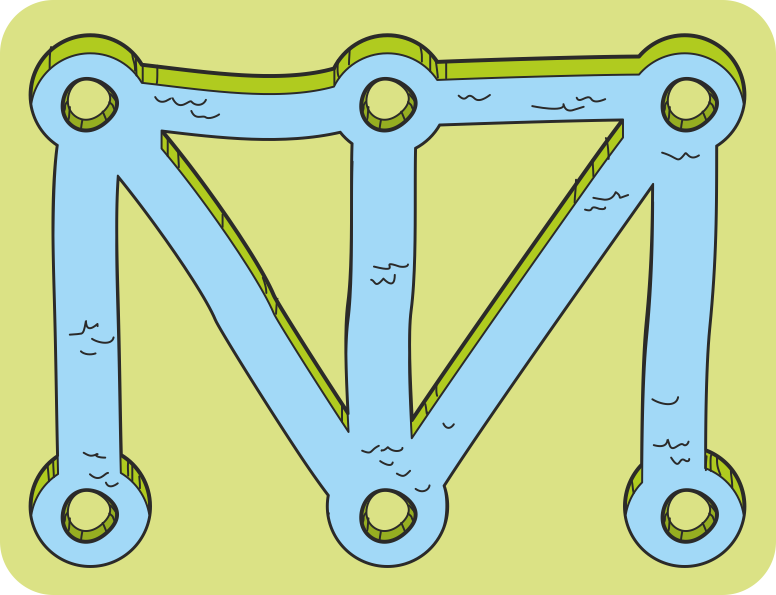
\includegraphics[width=1.0 \columnwidth]{figures/map_example.png}
    \caption{Example of a Map} 
    \label{fig:map} 
\end{figure}

\section{Levels and Goals}
\label{section:assignment}

The goal of this exercise set is to train the student's capability to find strategies to cover a graph with towers while minimizing the resources needed to do so. The users are encouraged to reflect on different positions where towers could be placed and how useful a particular drop zone is. 

On the first level, the students are required to check the placed towers whether they fulfil the condition that all channels can be observed. Often, there are channels that seem to be observed but are not since there is no adjacent tower.  

The second level then assigns a construction task to the students. They have to place a given number of towers onto the islands, such that all channels can be observed. For each map, the number of towers is set individually such that the task can be solved. Also, the number is kept small enough to prevent the user from placing a tower on every single island, which would be a trivial solution. The user has to find a permissible solution by him- or herself, and has to find ways to cover all the channels by trying out different approaches.

On the third level, the task is to find an optimal solution. The number of towers for an optimal solution is not explicitly mentioned, and thus one is required to find strategies to cover as many channels as possible with a single tower. The user is encouraged to consider and compare multiple solutions and evaluate them according to the given criterion.


\section{Implementation}
\label{section:implementation}
The implementation of the task levels is based on a game template and on a map template. The game template is called Towers.vue and defines the main structure and design. It also specifies the meta functionality like game generation, restart, and evaluation. The map template called TowersTemplate.vue then specifies the particular functions for a map that is then dynamically injected into the game template. In Towers.vue, there is additionally a \nameref{subsection:statementcheck} that is rendered below the component that contains the maps.

Each map has an underlying graph that is modelled according to the graph drawn on the map. This graph is modelled as an adjacency list and is based on a graph class providing all needed graph operations. The graph class can represent any directed or undirected graph and modify it by adding or removing edges and vertices.

%TC:ignore
\begin{lstlisting}[language=TypeScript,caption={},label={lst:graphClass}]
 class Graph {
  numberOfVertices;

  adjList;

  visitedNodes = new Set();

  queue = [0];

  constructor(vertices:number) {
    this.numberOfVertices = vertices;
    this.adjList = new Map();
  }
\end{lstlisting}
%TC:endignore

The testing is run over every solution proposition, independent if it was created by the computer or the user. The test checks if the proposition complies with all the regulations and consists of an algorithm that checks if the chosen vertex set forms a vertex cover. As a first step, all chosen vertices (contained in the array called arr) of the underlying graph are removed, including all incident edges (see code below). If the solution is correct, the towers cover all channels. When every vertex with a tower is removed, along with all edges symbolizing the channels, no edge or channel remains in the modified graph. The verification algorithm can be seen below in a simplified version:

\newpage
%TC:ignore
\begin{lstlisting}[language=TypeScript,caption={},label={lst:isVertexCover}]
  isVertexCover(arr:unknown[]):boolean {
    for (let i = 0; i < arr.length; i += 1) {
      removeVertex(Number(arr[i]));
    }

    const solution = isEmptyGraph();
    return solution;
  }
\end{lstlisting}
%TC:endignore

In a second step, the modified graph is tested on remaining edges. If the graph contains no edges, the solution is marked to be correct and permissible. 

%TC:ignore
\begin{lstlisting}[language=TypeScript,caption={},label={lst:isEmptyGraph}]
 isEmptyGraph():boolean {
    let empty = true;
    const getKeys = adjList.keys();
    for (const i of getKeys) {
      if (adjList.get(i).size > 0) {
        empty = false;
      }
    }
    return empty;
  }
\end{lstlisting}
%TC:endignore

The correctness of the level 1 proposition is immediately verified by the vertex cover algorithm when a random set is generated. Whenever the verify button is clicked, all the program does is comparing the user input to the result of the aforementioned algorithm.

The second level is reviewed by the verification algorithm as soon as the user has finished an own proposition and validates it. A solution is permissible if and only if the algorithm outputs true. 

Level 3 corresponds to the optimization task. Therefore, not only the regular checks as in level 2 are run, but also the optimality check is executed, which simply compares the number of used towers to the number of towers used in the optimal solution. Whenever both checks are evaluated positively, the result is emitted and marked as true.